\documentclass{report}
\usepackage{float}

% for the image in the title
\usepackage{tikz}

% custom spacing
\usepackage{setspace}
\onehalfspacing

% footer and header
\usepackage{fancyhdr}
% \setlength{\headheight}{15.2pt}

% underlining
\usepackage{ulem}


% Table of contents link to corresponding sections
\usepackage{hyperref}
\hypersetup{
	colorlinks,
	citecolor=black,
	filecolor=black,
	linkcolor=black,
	urlcolor=black
}

\usepackage{amsmath}
% Remove che "Chapter" string before chapters
\iffalse
\makeatletter
\def\@makechapterhead#1{%
	\vspace*{50\p@}%
	{\parindent \z@ \raggedright \normalfont
		\interlinepenalty\@M
		\Huge\bfseries  \thechapter.\quad #1\par\nobreak
		\vskip 40\p@
}}
\makeatother
\fi

% Fancy chapters
\usepackage[Bjarne]{fncychap}
% options: Sonny, Lenny, Glenn, Conny, Rejne, Bjarne, Bjornstrup

\begin{document}
	
	
	%title page
	\begin{titlepage}
		\begin{figure}[t]
			\centering
\includegraphics[width=0.3\textwidth]{images/unitn-logo}
		\end{figure}
		\begin{center}
			\textsc{ \LARGE{Università degli Studi di Trento \\}}
			\textsc{ \LARGE{Facoltà di Informatica\\ }}
			\textnormal{ \LARGE{Corso di Ingegneria del Software\\}}
			\vspace{30mm}
			\fontsize{10mm}{7mm}\selectfont 
			\textup{Fix Mi \\ Documento di Architettura}\\
		\end{center}
		
		\vspace{25mm}
		
		\centering
		\large Gruppo G43: \\ Giovanni Santini\\ Riginel Ungureanu \\ Valerio Asaro
		
		\vspace{20mm}
		
		\centering{\large{Anno Accademico 2023/2024 \\ Trento }}
		
	\end{titlepage}
	
	
	
	
	% use header and footers
	\pagestyle{fancy}
	\fancyhead[R]{\chaptername\ \thechapter}  % header
	
	%\maketitle
	\tableofcontents
	\newpage
	
	
	
	\section{Scopo del documento}
	
	Scadenza: 27 Novembre
	
	
	
	\section{Informazioni del Documento}
	
	% table
	\begin{center} % center the table
		\centering
		\begin{tabular}{ |p{4cm}|p{4cm}|  }
			\hline
			\centering Campo & \qquad\qquad Valore \\ % I found no other way...
			\hline
			Titolo del Documento & Documento di Architettura \\
			\hline
			Titolo del Progetto & Fix Mi \\
			\hline
			Autori del Documento &
			Giovanni Santini \\ & Riginel Ungureanu \\ & Valerio Asaro \\
			\hline
			Amministratore Progetto & Riginel Ungureanu\\
			\hline
			Versione del documento & 1.0 \\
			\hline
		\end{tabular}
	\end{center}
	
	
	
\chapter{Diagramma delle Classi}

In questa sezione dobbiamo partire dal diagramma dei componenti, dove "ogni componente diventa una classe"
Se ci vengono delle classi troppo grandi o con dati dirondanti vuol dire che dobbiamo splittarle in classi più piccole.


\section{Enumerazioni}
\begin{figure}[H]
	\centering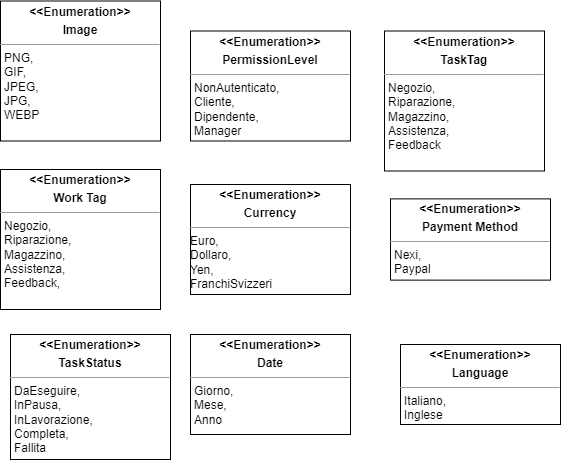
\includegraphics[width=1\textwidth]{images/Diagramma_delle_classi_Enumi.png}
	Diagramma delle classi per le Enumerazioni
\end{figure}
Allo scopo di definire dei tipi di dato chiari e comprensibili, sono state aggiunte le Enumerazioni di cui sotto:
\subsection*{Image}
L'Enumerazione Image rappresenta i diversi formati di immagine utilizzati all'interno dell'applicazione.
\subsection*{PermissionLevel}
L'Enumerazione PermissionLevel rappresenta il livello di permesso di un certo utente
\subsection*{TaskTag}
L'Enumerazione TaskTag rappresenta i vari tipi di TaskTag dell'applicazione
\subsection*{WorkTag}
L'Enumerazione WorkTag rappresenta i vari tipi di WorkTag dell'applicazione
\subsection*{Currency}
L'Enumerazione Currency rappresenta le valute supportate all'interno dell'applicazione
\subsection*{Payment Method}
L'Enumerazione Payment Method rappresenta le piattaforme di pagamento utilizzabili all'interno dell'applicazione 
\subsection*{TaskStatus}
L'Enumerazione TaskStatus rappresenta lo stato di una determinata task.
\subsection*{Date}
L'Enumerazione Date rappresenta una data
\subsection*{Language}
L'Enumerazione Language rappresenta una lingua supportata dall'applicazione

\section{Microservizio}
\begin{figure}[H]
	\centering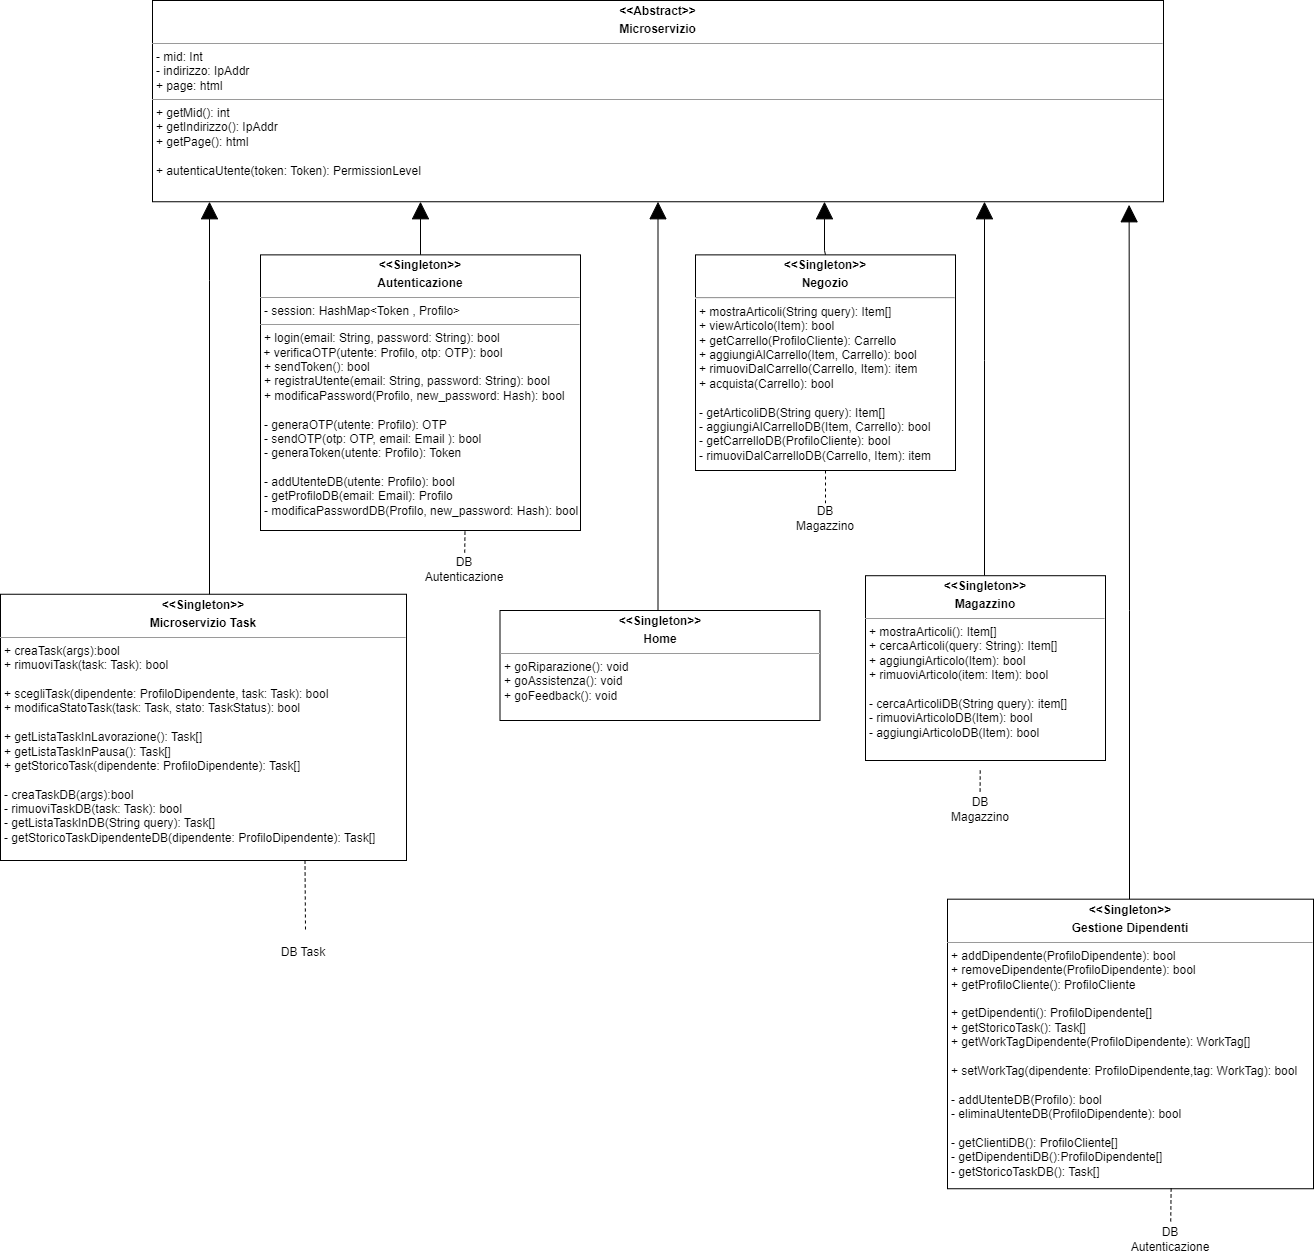
\includegraphics[width=1\textwidth]{images/Diagramma_delle_classi_Microservizio.png}
	Diagramma delle classi per i Microservizi
\end{figure}
Data la specifica del Back-End e dato il diagramma di contesto sono state individuate le classi e relativi metodi e attributi di cui sotto
\subsection*{Descrizione}
La classe astratta Microservizio rappresenta un microservizio generico dell'applicazione.
A questi fini sono stati identificati i seguenti attributi e metodi
\begin{itemize}
	\item private mid: Int 
	\begin{itemize}
		\item questo attributo è un codice identificativo univoco per il microservizio.
	\end{itemize}
	\item private indirizzo: IpAddr
	\begin{itemize}
		\item questo attributo corrisponde all'indirizzo IP e porta del microservizio.
	\end{itemize}
	\item public page: html
	\begin{itemize}
		\item questo attributo contiene la pagina principale del microservizio in html 
	\end{itemize}
	
	\item public autenticaUtente(token: Token): PermissionLevel 
	\begin{itemize}
		\item il metodo permette di richiedere al "microservizio autenticazione" il livello di permesso di un determinato utente, che ha fornito il suo token di sessione. ritorna il PermissionLevel dell'utente.
	\end{itemize}
\end{itemize}
\subsection*{Classi figlie}
Le classi figlie di "Microservizio" sono singleton, ciascuna rappresentante uno specifico microservizio dell'applicazione.
Queste sono le seguenti:
\begin{itemize}
	\item Microservizio Task
	\item Autenticazione
	\item Negozio
	\item Home
	\item Magazzino
	\item Gestione Dipendenti
\end{itemize}

\section{Database}
\begin{figure}[H]
	\centering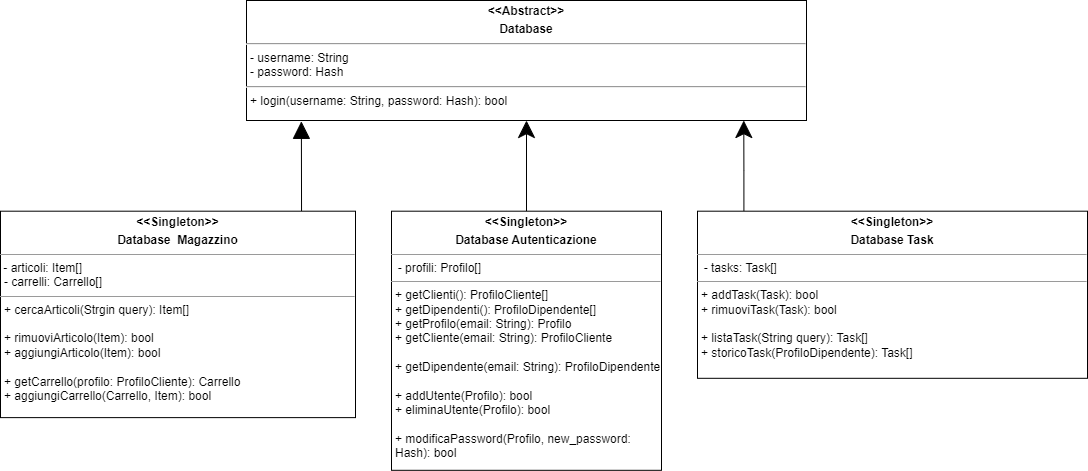
\includegraphics[width=1\textwidth]{images/Diagramma_delle_classi_Database.png}
	Diagramma delle classi per i Database
\end{figure}
Data la specifica del Back-End e il diagramma di Contesto sono state individuate le classi e relativi metodi e attributi di cui sotto:
\subsection*{Descrizione}
La classe astratta Database rappresenta un Database generico dell'applicazione.
A questi fini sono stati identificati i seguenti attributi e metodi
\begin{itemize}
	\item private username: String 
	\begin{itemize}
		\item questo attributo è l'username necessario per accedere al database
	\end{itemize}
	\item private password: Hash 
	\begin{itemize}
		\item questo attributo è l'Hash della password necessaria per accedere al database
	\end{itemize}
	\item public login(username: String, password: Hash): bool 
	\begin{itemize}
		\item questo metodo permette a un utente o a un microservizio di accedere al database per eseguire le proprie query. ritorna true se l'operazione è andata a buon fine, false altrimenti
	\end{itemize}
\end{itemize}
\subsection*{Classi figlie}
Le classi figlie di Database sono singleton, ciascuna rappresenta un specifico database dell'applicazione. 
Questi sono: 
\begin{itemize}
	\item Database Magazzino
	\item Database Autenticazione
	\item Database Task
\end{itemize}
\section{Profilo}
\begin{figure}[H]
	\centering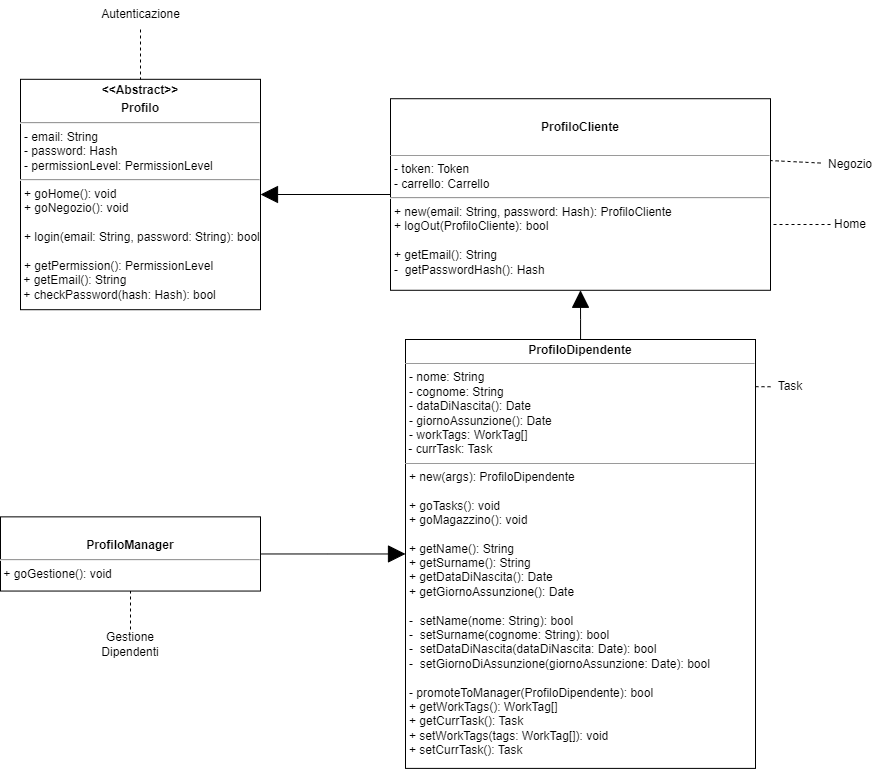
\includegraphics[width=1\textwidth]{images/Diagramma_delle_classi_Profilo.png}
	Diagramma delle classi per i profili
\end{figure}
Data l'analisi del Contesto sezione 1 "Utenti e Sistemi Esterni"  sono state individuate le classi e relativi metodi e attributi di cui sotto:
\subsection*{Descrizione}
La classe astratta Profilo rappresenta il profilo di un utente del sistema che ha eseguito l'autenticazione.
L'utente autenticato nel proprio profilo può utilizzare le funzionalità del sistema attraverso i microservizi, e può visitare le varie pagine in base al proprio PermissionLevel. 
A questi fini sono stati identificati i seguenti metodi e attributi:
\begin{itemize}
	\item private email: String
	\begin{itemize}
		\item questo attributo è l'email appartenente all'utente
	\end{itemize}
	\item private password: Hash 
	\begin{itemize}
		\item questo attributo è l'Hash della password dell'utente
	\end{itemize}
	\item private permissionLevel: PermissionLevel 
	\begin{itemize}
		\item questo attributo è il livello di permesso dell'utente
	\end{itemize}
	\item public goHome(): void 
	\begin{itemize}
		\item questo metodo permette all'utente di andare alla pagina Home
	\end{itemize}
	\item public goNegozio(): void 
	\begin{itemize}
		\item questo metodo permette all'utente di andare alla pagina Negozio
	\end{itemize}
	\item public checkPassword(hash: Hash): bool 
	\begin{itemize}
		\item questo attributo compara l'attributo password con l'hash fornito, ritornando true se combaciano, false altrimenti
	\end{itemize}
\end{itemize}
\subsection*{ProfiloCliente}
La classe ProfiloCliente, figlia della classe "Profilo" rappresenta il profilo di un cliente
Sono stati identificati i seguenti metodi e attributi: 
\begin{itemize}
	\item private token: Token
	\begin{itemize}
		\item questo attributo rappresenta il token di sessione di un cliente
	\end{itemize}
	\item private carrello: Carrello
	\begin{itemize}
		\item questo attributo rappresenta il carrello del cliente.
	\end{itemize}
	\item public new(email: String, password: Hash): ProfiloCliente
	\begin{itemize}
		\item questo metodo permette di creare un nuovo ProfiloCliente contenenti l'email e l'hash password forniti.
	\end{itemize}
	\item public logOut(profilo: ProfiloCliente): bool
	\begin{itemize}
		\item questo metodo permette di eseguire il logOut dall'applicazione, ritorna true se l'operazione è stata eseguita con successo, false altrimenti
	\end{itemize}
\end{itemize}
\subsection*{ProfiloDipendente}
La classe ProfiloDipendente, figlia della classe "ProfiloCliente" rappresenta il profilo di un dipendente dell'azienda.
Sono stati identificati i seguenti metodi e attributi: 
\begin{itemize}
	\item private workTags: WorkTag[]
	\begin{itemize}
		\item questo attributo rappresenta una lista di workTag del dipendente.
	\end{itemize}
	\item private promoteToManager(profiloDipendente): bool
	\begin{itemize}
		\item questo metodo permette di trasformare il profiloDipendente fornito in un profiloManager
	\end{itemize}
\end{itemize}
\subsection*{ProfiloManager}
La classe ProfiloManager, figlia della classe "ProfiloDipendente" rappresenta il profilo del manager dell'azienda.



\section{Autenticazione}

\begin{figure}[H]
	\centering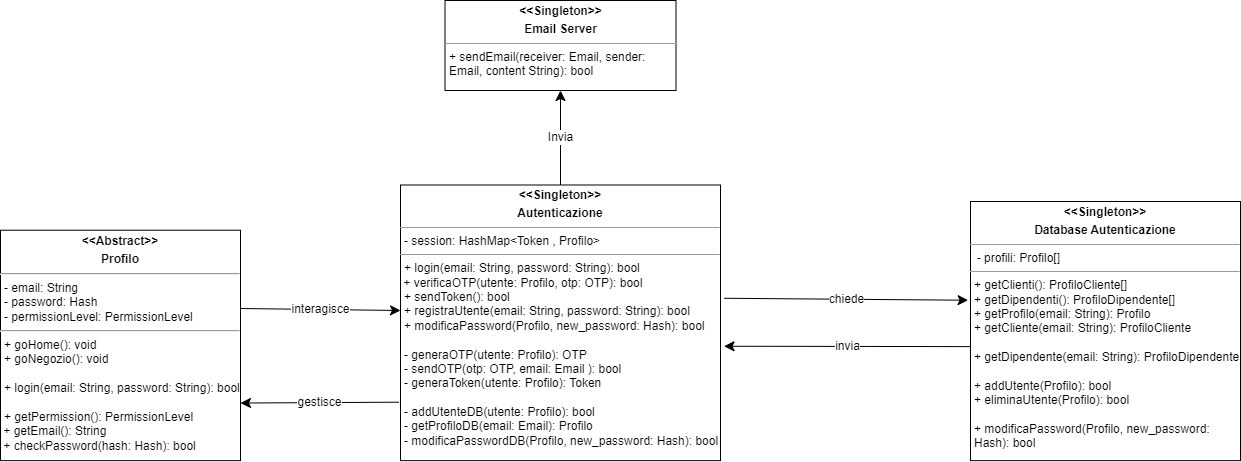
\includegraphics[width=1\textwidth]{images/Diagramma_delle_classi_Autenticazione.png}
	Diagramma delle classi per la componente "Autenticazione" 
\end{figure}

Date le seguenti componenti: 
\begin{itemize}
	\item "Autenticazione"
	\item "Login"
	\item "Registrazione"
	\item "Cambio Password"
\end{itemize}
seguendo ciò che è stato descritto negli RF "1" e "2" sono state individuate le classi e relativi metodi e attributi di cui sotto:
\subsection{Descrizione}
La classe "Autenticazione" è un singleton che rappresenta il microservizio avente lo stesso nome. 
Questa classe gestisce i dati di autenticazione dei profili quali e-mail, password e token. 
La classe contiene una HashMap che associa a ogni profilo un Token identificativo per la sessione.
A questi fini, sono stati identificati i seguenti metodi:
\begin{itemize}
	\item public login( email: String, password: String ) : bool
		\begin{itemize}
			\item questo metodo permette a un utente di eseguire il login, ritornando true se è avvenuto con successo e false altrimenti
			\item all'interno del metodo, dopo aver eseguito il controllo dell'esistenza di un profilo con stessa email e password,
			viene generato un codice 2FA e inviato alla email rispettiva utilizzando i metodi "generaOTP()" e "sendOTP()", per poi aspettare che l'utente lo inserisca
			\item alla fine del metodo e in caso di esito positivo, un token viene generato , inserito nella session e inviato all'utente utilizzando i metodi generaToken() e sendToken() rispettivamente
		\end{itemize}
	\item public verificaOTP( utente: Profilo, otp: OTP): bool
		\begin{itemize}
			\item questo metodo è necessario per verificare l'identità dell'utente attraverso il codice OTP, ritornando true se l'OTP inserito è giusto.
		\end{itemize}
	\item public sendToken() :bool 
		\begin{itemize}
			\item questo metodo permette di inviare ad un utente il suo token
		\end{itemize}
	\item public registraUtente(email: String, password: String): bool
		\begin{itemize}
			\item questo metodo permette ad un nuovo utente di registrarsi, ritornando true se la registrazione è andata a buon fine
			\item all'interno del metodo, dopo aver controllato che l'email fornita non appartenga a un profilo esistente, viene generato un codice 2FA e inviato alla email rispettiva utilizzando i metodi "generaToken()" e "sendToken()", per poi aspettare che l'utente lo inserisca
		\end{itemize}
	\item public modificaPassword(Profilo, new\_password: Hash ) :bool
		\begin{itemize}
			\item questo metodo permette ad un utente di modificare la propria password, fornendo l'hash della nuova password, e ritorna true se la modifica è andata buon fine, false altrimenti
			\item all'interno del metodo viene generato un codice 2FA e inviato alla email rispettiva utilizzando i metodi "generaToken()" e "sendToken()", per poi aspettare che l'utente lo inserisca
		\end{itemize}
	\item private generaOTP(utente: Profilo) : OTP
		\begin{itemize}
			\item questo metodo genera un codice OTP per un profilo, ritornandolo 
		\end{itemize}
	\item private sendOTP(otp: OTP, email: Email): bool
		\begin{itemize}
			\item questo metodo invia un codice OTP alla email fornita, ritornando true se l'operazione è andata a buon fine, false altrimenti
		\end{itemize}
	\item private generaToken(utente: Profilo) : Token
		\begin{itemize}
			\item questo metodo genera un token per un determinato utente, inserendolo nella session e ritornandolo
		\end{itemize}
	\item private addUtenteDB(utente:Profilo): bool
		\begin{itemize}
			\item questo metodo chiede al DB di aggiungere un nuovo profilo utente 
		\end{itemize}
	\item private getProfiloDB(email: Email) : Profilo
		\begin{itemize}
			\item questo metodo chiede al DB il profilo avente la mail fornita. Se esiste viene ritornato il profilo, altrimenti null
		\end{itemize}
	\item private modificaPasswordDB(profilo: Profilo, new\_password: Hash) : bool
		\begin{itemize}
			\item questo metodo richiede al DB la modifica della password di un dato profilo, e ritorna true se il processo è andato a buon fine, false altrimenti
		\end{itemize}
\end{itemize}
\subsection*{Database Autenticazione}
La classe Database Autenticazione è un singleton che rappresenta il database contenente i profili. 
Permette di gestire i profili, aggiungerli ed eliminarli.
Sono stati individuati i seguenti metodi: 
\begin{itemize}
	\item public getClienti(): ProfiloCliente[]
	\begin{itemize}
		\item questo metodo ritorna tutti i profili cliente immagazinati
	\end{itemize}
	\item public getDipendenti(): ProfiloDipendente[]
	\begin{itemize}
		\item questo metodo ritorna tutti i profili dipendente immagazinati
	\end{itemize}
	\item public getProfilo(email: String): Profilo
	\begin{itemize}
		\item questo metodo ritorna il profilo a cui corrisponde l'email fornita. Se non esiste ritorna null
	\end{itemize}
	\item public getCliente(email: String): ProfiloCliente
	\begin{itemize}
		\item questo metodo ritorna il profilo cliente a cui corrisponde l'email fornita. se non esiste ritorna null
	\end{itemize}
	\item public getDipendente(email String): ProfiloDipendente
	\begin{itemize}
		\item questo metodo ritorna il profilo dipendente a cui corrisponde l'email fornita. se non esiste ritorna null
	\end{itemize}
	\item public addUtente(profilo: Profilo): bool
	\begin{itemize}
		\item questo metodo inserisce il profilo fornito nel database. ritorna true se l'operazione è avvenuta con successo, false altrimenti
	\end{itemize}
	\item public eliminaUtente(profilo: Profilo): bool
	\begin{itemize}
		\item questo metodo elimina il profilo fornito dal database. ritorna true se l'operazione è avvenuta con successo, false altrimenti
	\end{itemize}
	\item public modificaPassword(profilo: Profilo, new\_password: Hash): bool
	\begin{itemize}
		\item questo metodo modifica la password immagazzinata nel database del profilo fornito. ritorna true se l'operazione è avvenuta con successo, false altrimenti
	\end{itemize}
\end{itemize}
\subsection*{Email Server}
La classe Email Server è un singleton che rappresenta il server email utilizzato dall'azienda. permette di inviare email.
Sono stati individuati i seguenti metodi:
\begin{itemize}
	\item public sendEmail(receiver: Email, sender: Email,content: String) : bool
	\begin{itemize}
		\item questo metodo invia una mail dall'email del mittente(sender) all'email del destinatario(receiver) con il contenuto(content)
	\end{itemize}
\end{itemize}
\subsection*{Profilo}
La classe astratta Profilo rappresenta il profilo di un determinato utente. Viene gestito dal microservizio Autenticazione e immagazzinato nel database Autenticazione.
Sono stati individuati i seguenti metodi:
\begin{itemize}
	\item public login(email: String, password: Hash) : bool
	\begin{itemize}
		\item questo metodo permette a un utente di svolgere il login nel proprio profilo, fornendo l'email e la password. restituisce true se l'operazione è andata a buon fine, false altrimenti
	\end{itemize}
\end{itemize}
\chapter{Codice in Object Constraint Language}	
In questo capitolo è descritta in modo formale la logica prevista nell’ambito di alcune operazioni di alcune classi.
Tale logica viene descritta in Object Constraint Language (OCL) perché tali concetti non sono esprimibili in nessun altro modo formale nel contesto di UML.	
\section{Microservizio Task}
\begin{figure}[H]
	\centering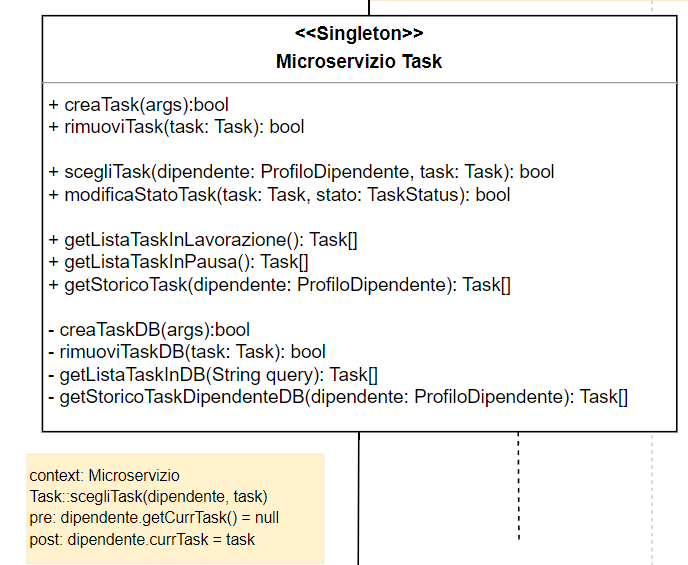
\includegraphics[width=1\textwidth]{images/OCL/OCL_task.png}
	Diagramma delle classi con linguaggio OCL 
\end{figure}
Quando un dipendente sceglie una task su cui lavorare non deve avere nessuna task correntemente assegnata.
\begin{verbatim}
	context: Microservizio Task::scegliTask(dipendente, task)
	pre: dipendente.getCurrTask() = null
	post: dipendente.currTask = task

\end{verbatim}

\section{Carrello}
\begin{figure}[H]
	\centering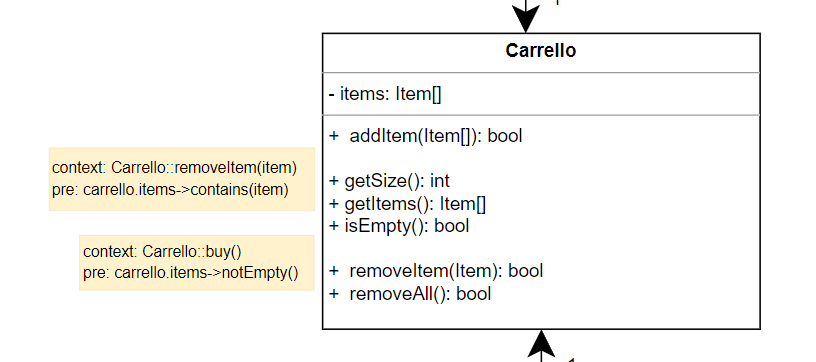
\includegraphics[width=1\textwidth]{images/OCL/OCL_carrello.png}
	Diagramma delle classi con linguaggio OCL 
\end{figure}
Per rimuovere un articolo da un carrello è necessario che quell'articolo faccia parte del carrello.
\begin{verbatim}
	context: Carrello::removeItem(item)
	pre: carrello.items->contains(item)

\end{verbatim}
Per comprare gli articoli del carrello è necessario che il carrello non sia vuoto
\begin{verbatim}
	context: Carrello::buy()
	pre: carrello.items->notEmpty()

\end{verbatim}

\section{Autenticazione}
\begin{figure}[H]
	\centering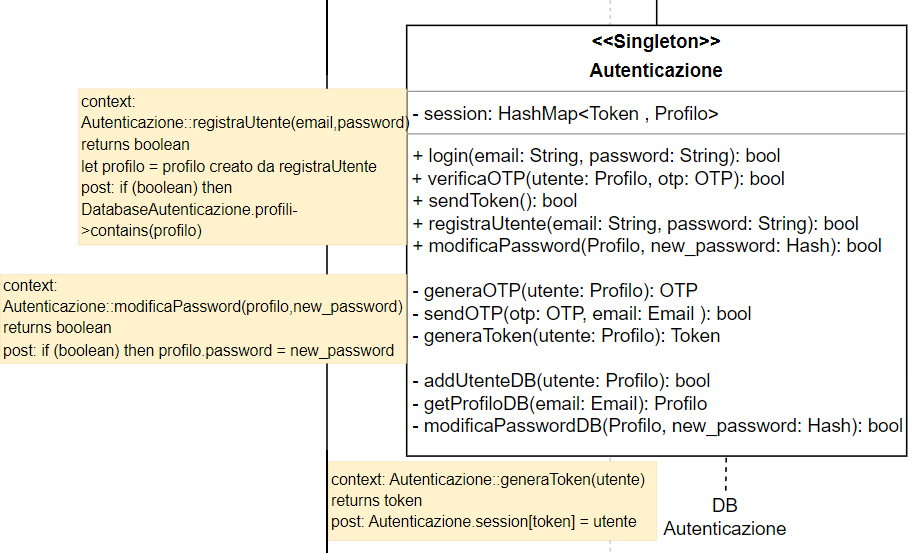
\includegraphics[width=1\textwidth]{images/OCL/OCL_Autenticazione.PNG}
	Diagramma delle classi con linguaggio OCL 
\end{figure}
una volta generato un Token utente, esso viene automaticamente inserito dentro alla session
\begin{verbatim}
	context: Autenticazione::generaToken(utente) returns token
	post: Autenticazione.session[token] = utente

\end{verbatim}
Una volta modificata la password di un profilo utente, allora la password contenuta all'interno dello stesso dev'essere quella nuova
\begin{verbatim}
	context: Autenticazione::modificaPassword(profilo,new_password) returns boolean
post: if (boolean) then profilo.password = new_password

\end{verbatim}
Una volta registrato un utente, il suo profilo deve apparire nel database
\begin{verbatim}
	context: Autenticazione::registraUtente(email,password) returns boolean
	let profilo = profilo creato da registraUtente
	post: if (boolean) then DatabaseAutenticazione.profili->contains(profilo)

\end{verbatim}
\section{Gestione Dipendenti}
\begin{figure}[H]
	\centering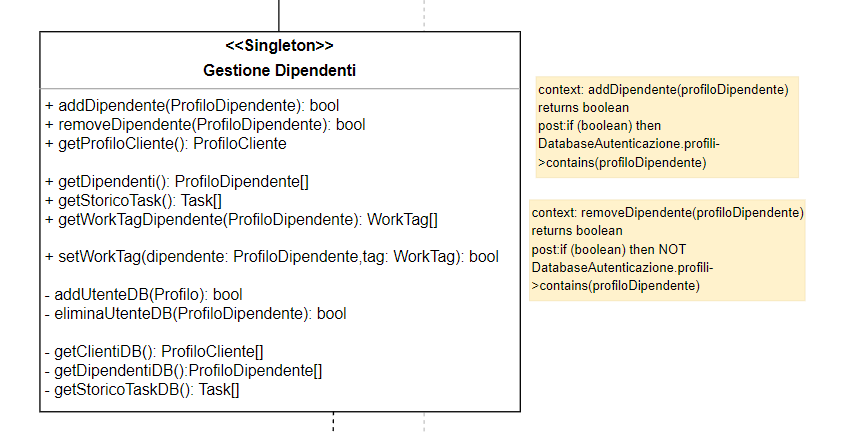
\includegraphics[width=1\textwidth]{images/OCL/OCL_Gestione_Dipendenti.PNG}
	Diagramma delle classi con linguaggio OCL 
\end{figure}
Una volta che un profilo dipendente viene aggiunto, deve apparire all'interno del database
\begin{verbatim}
	context: addDipendente(profiloDipendente) returns boolean
	post:if (boolean) then DatabaseAutenticazione.profili->contains(profiloDipendente)
\end{verbatim}
Una volta che un profilo dipendente viene rimosso, non deve più apparire all'interno del database
\begin{verbatim}
	context: removeDipendente(profiloDipendente) returns boolean
	post:if (boolean) then NOT DatabaseAutenticazione.profili->contains(profiloDipendente)

\end{verbatim}

\section{Negozio}
\begin{figure}[H]
	\centering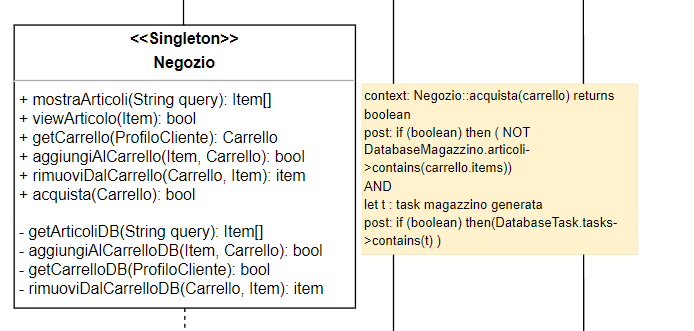
\includegraphics[width=1\textwidth]{images/OCL/OCL_negozio.png}
	Diagramma delle classi con linguaggio OCL 
\end{figure}
Una volta acquistati gli articoli, il database non deve più contenerli. Inoltre dev'essere creata una task magazzino.
\begin{verbatim}
	context: Negozio::acquista(carrello) returns boolean
	post: if (boolean) then ( NOT DatabaseMagazzino.articoli->contains(carrello.items))
	AND
	let t : task magazzino generata 
	post: if (boolean) then(DatabaseTask.tasks->contains(t) )
	
\end{verbatim}
\section{Assistenza, Riparazione, Feedback}
\begin{figure}[H]
	\centering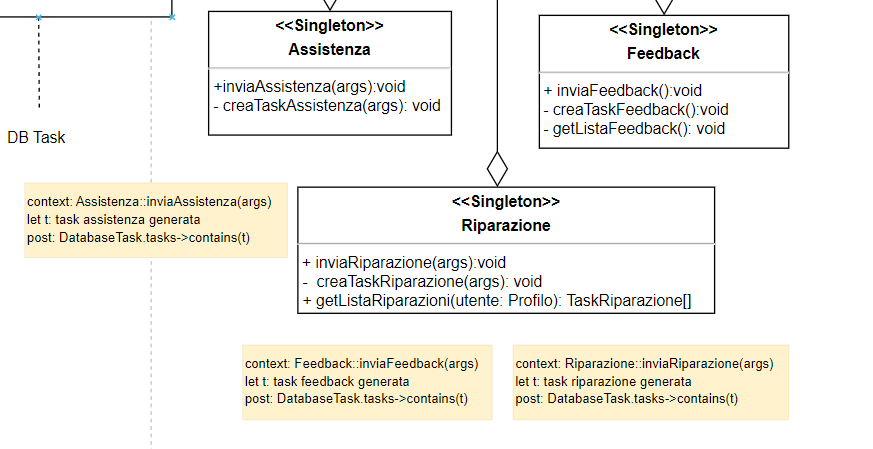
\includegraphics[width=1\textwidth]{images/OCL/OCL_assistenza_riparazione_feedback.PNG}
	Diagramma delle classi con linguaggio OCL 
\end{figure}
Una volta inviata una richiesta di assistenza, riparazione o feedback, viene creata la corrispettiva task e inserita nel database
\begin{verbatim}
	context: Assistenza::inviaAssistenza(args)
	let t: task assistenza generata
	post: DatabaseTask.tasks->contains(t)

	context: Feedback::inviaFeedback(args)
	let t: task feedback generata
	post: DatabaseTask.tasks->contains(t)

	context: Riparazione::inviaRiparazione(args)
	let t: task riparazione generata
	post: DatabaseTask.tasks->contains(t)

\end{verbatim}
\section{ProfiloDipendente, ProfiloCliente, ProfiloManager}
\begin{figure}[H]
	\centering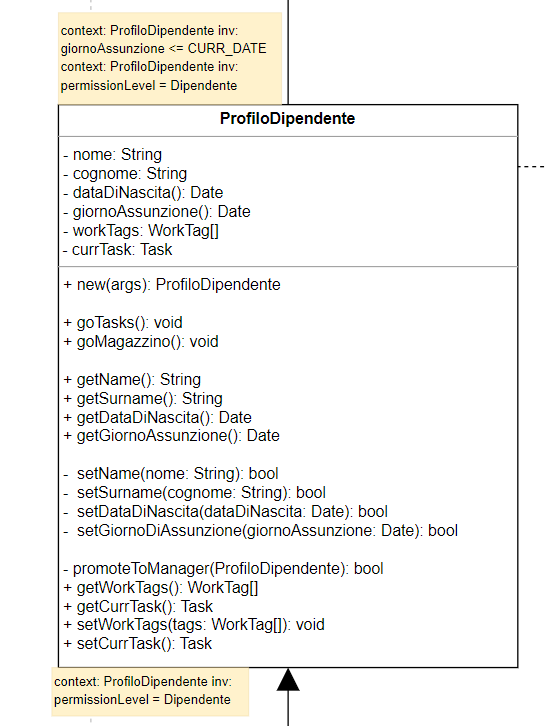
\includegraphics[width=1\textwidth]{images/OCL/OCL_dipendente.png}
	Diagramma delle classi con linguaggio OCL 
\end{figure}
\begin{figure}[H]
	\centering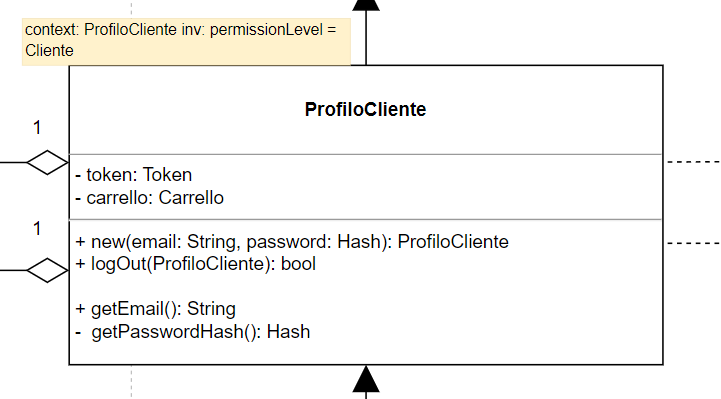
\includegraphics[width=1\textwidth]{images/OCL/OCL_cliente.png}
	Diagramma delle classi con linguaggio OCL 
\end{figure}
\begin{figure}[H]
	\centering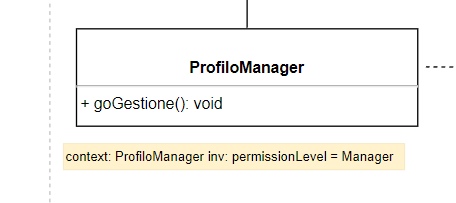
\includegraphics[width=1\textwidth]{images/OCL/OCL_manager.png}
	Diagramma delle classi con linguaggio OCL 
\end{figure}
La data d'assunzione del dipendente dev'essere inferiore a quella odierna
\begin{verbatim}
	context: ProfiloDipendente inv: giornoAssunzione <= CURR_DATE
\end{verbatim}
ProfiloDipendente, ProfiloCliente, ProfiloManager hanno i PermissionLevel rispettivi
\begin{verbatim}
	context: ProfiloDipendente inv: permissionLevel = Dipendente
	context: ProfiloCliente inv: permissionLevel = Cliente
	context: ProfiloManager inv: permissionLevel = Manager
\end{verbatim}

\chapter{Diagramma delle classi con codice OCL}
\begin{figure}[H]
	\centering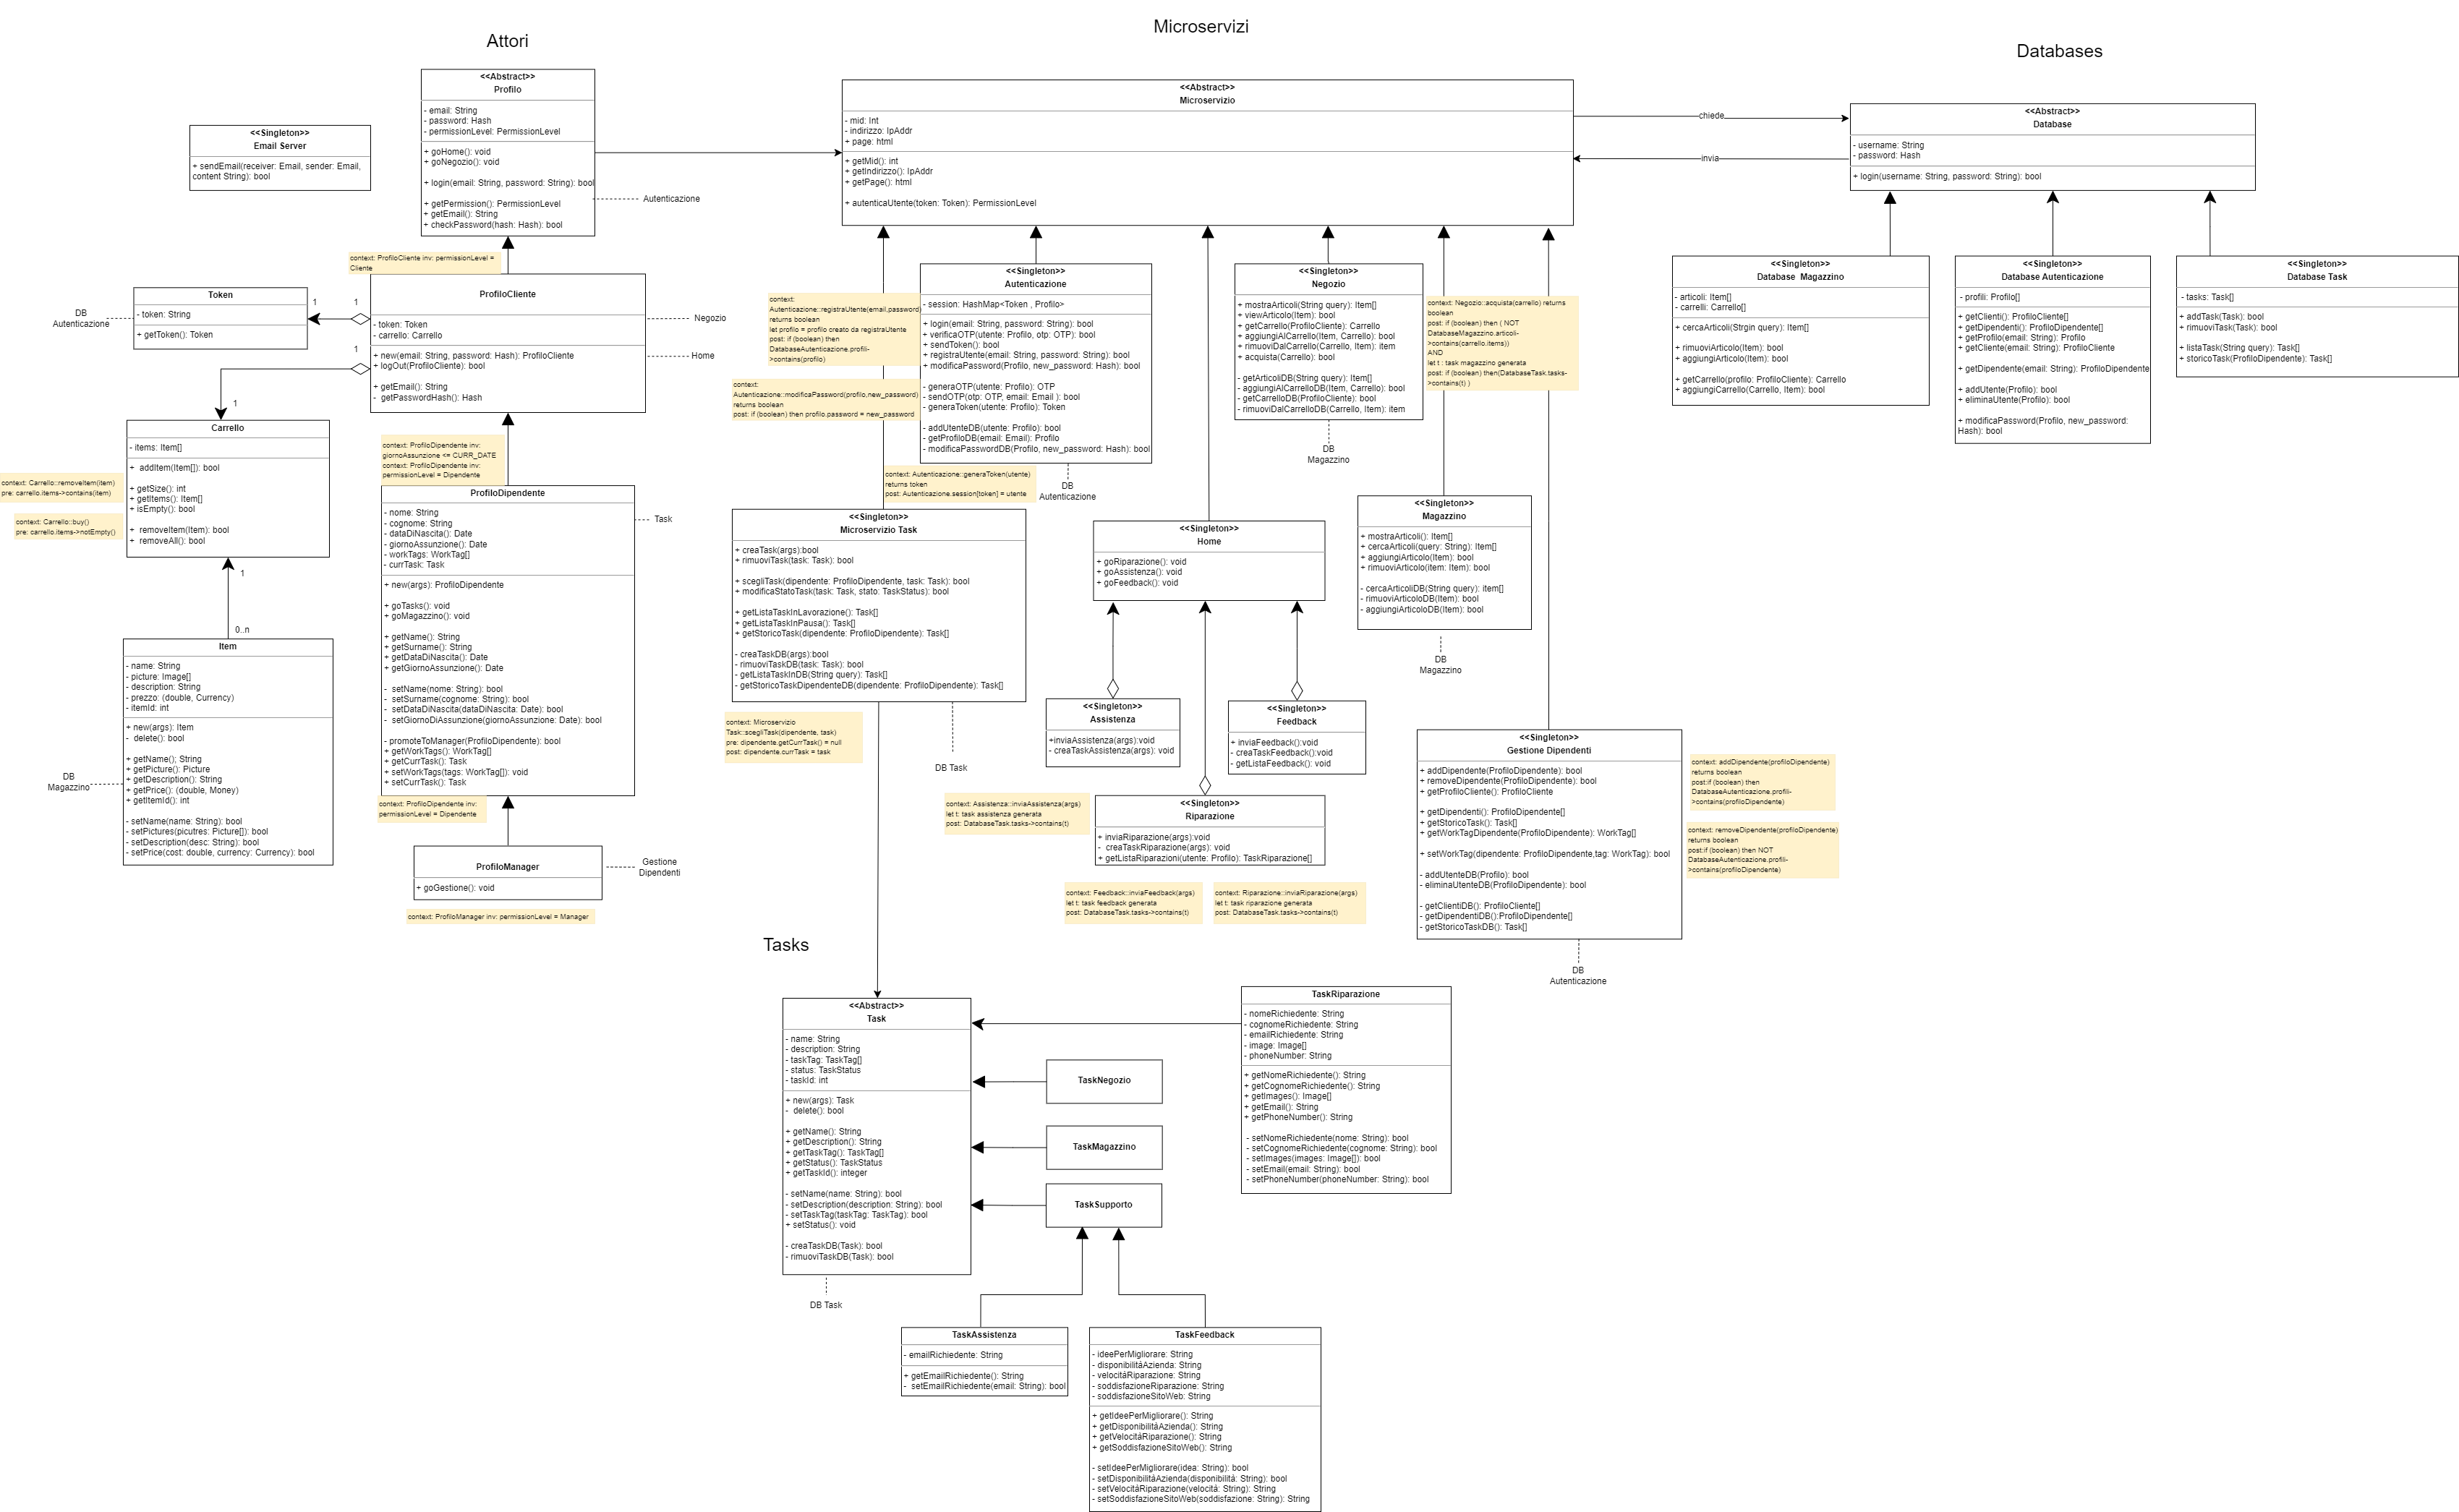
\includegraphics[width=1\textwidth]{images/Diagramma_delle_classi_OCL.png}
	Diagramma delle classi con linguaggio OCL 
\end{figure}
\end{document}